\documentclass[tikz,border=2pt]{standalone}
\usepackage{amsmath}
\usepackage{pgfplots}
\pgfplotsset{compat=1.18}
\usetikzlibrary{arrows.meta}
\begin{document}
% Example 2 (Example 3.4): V = {-2x1+x2<=6, x1+x2<=3, 3x1-x2<=5}, f(x)=-x1-x2 with minimum m=-3 on V;
% the minimizers form V cap H, H={x1+x2=3}, the segment from (-1,4) to (2,1); (1/2,5/2) is a minimizer, not extreme.
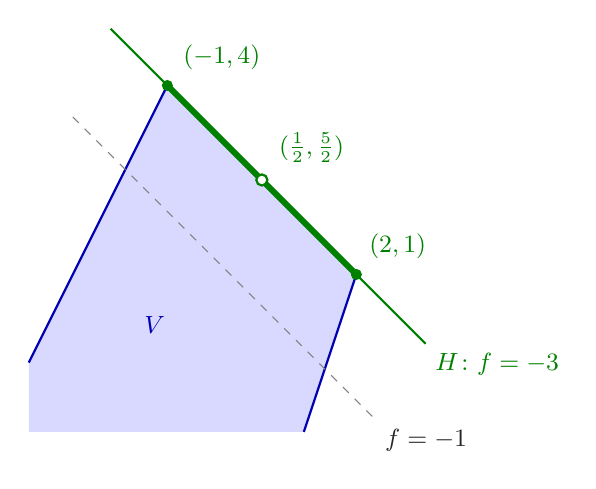
\begin{tikzpicture}[font=\small, >={Latex[length=2mm]}]
  \begin{scope}[x=0.8cm, y=0.8cm]
    \fill[blue!15] (-1,4) -- (2,1) -- ({7/6},-1.5) -- (-3.2,-1.5) -- (-3.2,-0.4) -- cycle;
    \draw[blue!70!black, thick] (-3.2,-0.4) -- (-1,4) (2,1) -- ({7/6},-1.5);
    \node[blue!70!black] at (-1.2,0.2) {$V$};
    \draw[gray, thin, dashed] (-2.5,3.5) -- (2.3,-1.3);
    \node[gray!30!black, anchor=north west] at (2.3,-1.3) {$f=-1$};
    \draw[green!50!black, thick] (-1.9,4.9) -- (3.1,-0.1);
    \draw[green!50!black, line width=2.2pt] (-1,4) -- (2,1);
    \node[green!50!black, anchor=north west] at (3.1,-0.1) {$H\colon f=-3$};
    \fill[green!50!black] (-1,4) circle (2pt) (2,1) circle (2pt);
    \draw[green!50!black, thick, fill=white] (0.5,2.5) circle (2pt);
    \node[green!50!black, anchor=south west] at (-0.9,4.1) {$(-1,4)$};
    \node[green!50!black, anchor=south west] at (2.05,1.1) {$(2,1)$};
    \node[green!50!black, anchor=south west] at (0.62,2.62) {$(\tfrac{1}{2},\tfrac{5}{2})$};
  \end{scope}
\end{tikzpicture}
\end{document}
